% !TeX root = ../Book3.tex
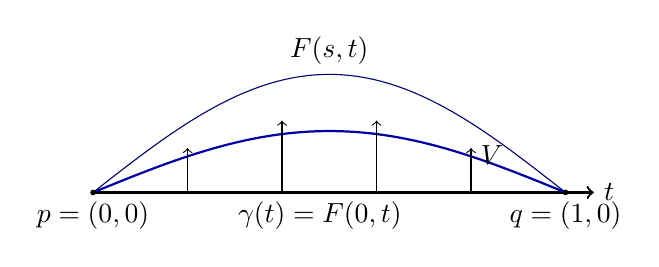
\begin{tikzpicture}[x=6cm,y=1.2cm]
	\draw[thick,->] (0,0)--(1.06,0) node[right] {\(t\)};
	\draw[blue!65!black,thick,domain=0:1,samples=60] plot (\x,{0.65*sin(180*\x)});
	\draw[blue!45!black,domain=0:1,samples=60] plot (\x,{1.25*sin(180*\x)});
	\foreach \x in {0.2,0.4,0.6,0.8}{
		\draw[->] (\x,0)--(\x,{0.8*sin(180*\x)});
	}
	\fill (0,0) circle[x radius=.006,y radius=.03];
	\fill (1,0) circle[x radius=.006,y radius=.03];
	\node[below] at (0,0) {\(p=(0,0)\)};
	\node[below] at (1,0) {\(q=(1,0)\)};
	\node[below] at (.48,0) {\(\gamma(t)=F(0,t)\)};
	\node[above] at (.5,1.25) {\(F(s,t)\)};
	\node[right] at (.8,.4) {\(V\)};
\end{tikzpicture}
